\documentclass{article}
\usepackage[final]{neurips_2020}

\usepackage[utf8]{inputenc} % allow utf-8 input
\usepackage[T1]{fontenc}    % use 8-bit T1 fonts
\usepackage{hyperref}       % hyperlinks
\usepackage{url}            % simple URL typesetting
\usepackage{booktabs}       % professional-quality tables
\usepackage{amsfonts}       % blackboard math symbols
\usepackage{nicefrac}       % compact symbols for 1/2, etc.
\usepackage{microtype}      % microtypography

\usepackage[pdftex]{graphicx} % include images
\usepackage{amsmath}          % for multi-line equations
\usepackage{bbm}              % for the indicator function \bbm{1}
\usepackage{multirow}         % for multi-row table cells
\usepackage{subcaption}       % for subfigures
\usepackage{pgffor}           % for the \foreach loop
\usepackage{ifthen}           % for the \ifthenelse statement

\setcitestyle{numbers,square}
\bibliographystyle{plainnat}

% Common values referred throughout the text
\newcommand{\defmoepochs}{7}
\newcommand{\oursepochs}{4}
\newcommand{\defmobatchsize}{24}
\newcommand{\oursbatchsize}{9}

\title{Improving DeFMO With Learned Losses}

% The \author macro works with any number of authors. There are two commands
% used to separate the names and addresses of multiple authors: \And and \AND.
%
% Using \And between authors leaves it to LaTeX to determine where to break the
% lines. Using \AND forces a line break at that point. So, if LaTeX puts 3 of 4
% authors names on the first line, and the last on the second line, try using
% \AND instead of \And before the third author name.
\author{%
    Harish Rajagopal \\
    Computer Science MSc \\
    ETH Zürich \\
    20-946-349 \\%chktex 8
    \AND%
    Denys Rozumnyi \\
    Co-Supervisor \\
    Department of Computer Science \\
    ETH Zürich \\
    \And%
    Prof.\ Dr.\ Marc Pollefeys \\
    Supervisor \\
    Department of Computer Science \\
    ETH Zürich
}

\begin{document}

\maketitle

\begin{abstract}

DeFMO is an algorithm that aims to remove motion blur in images using a neural network to deblur individual frames as well as generate `sub-frames', as if captured by a high-speed camera (i.e.\ temporal super-resolution).
This project extends DeFMO using Generative Adversarial Networks.
Our approach overcomes limitations within the loss formulation of DeFMO, more accurately captures the `quality' of the generated outputs, and thus improves results.
We also introduce a novel loss function for tackling temporal consistency among generated sub-frames.
Further, we optimize the codebase to be more memory-efficient, and improve readability and maintainability.

\end{abstract}

\section{Introduction}

Motion blur is a challenging problem in computer vision.
It occurs when moving objects are captured with long exposures.
This leads to a loss of information in images, and thus algorithms for deblurring are pursued.
Deblurring motion blur due to fast moving objects~\citep{fmo} (FMOs) is a challenging subset of this task, and it is necessary for tracking FMOs such as in ball-based sports, free-falling objects, high-speed cars, etc.

% TODO:
% * Cite all other deblurring papers
% * Extend into proper literature review
Various deep learning approaches have been proposed to tackle FMO blur.
\citet{defmo} proposed an algorithm known as DeFMO, that uses a convolutional encoder-decoder architecture to deblur individual images by generating sub-frames that depict the motion of the FMO.\@
The model is trained in a supervised learning setting with a wide variety of losses for good performance.

While these losses lead to good performance on various datasets, they might not be optimal for the best performance.
Here, we aim to replace these hand-engineered losses with neural networks that can learn a loss function for training the base model.
For this, we use Generative Adversarial Networks~\citep{gan} (GANs).

The \textbf{contributions} of this project are:
\begin{itemize}
    \item Improvement of the DeFMO model's outputs using GANs.
    \item A novel learned loss function for temporal frame consistency.
    \item A generalized approach over DeFMO for any task that involves video super-resolution.
    \item Optimizations for more efficient memory management during training.
    \item Refactoring and code quality enforcement over the DeFMO codebase.
\end{itemize}

\section{Baseline}

The baseline model is DeFMO.\@
Here, the input consists of an RGB image $I \in \mathbb{R}^{H \times W \times 3}$ of the foreground blurred FMO with height $H$ and width $W$, and another RGB Image $B \in \mathbb{R}^{H \times W \times 3}$ of the background.
The desired output is a deblurred rendering of the FMO for $N$ sub-frames.
The $t$\textsuperscript{th} sub-frame is an RGBA image $R_t \in \mathbb{R}^{H \times W \times 4}$ consisting of an RGB part $F_t \in \mathbb{R}^{H \times W \times 3}$ for the sharp appearance of the FMO, and an alpha matting mask $M_t \in \mathbb{R}^{H \times W}$ which segments the FMO from the background.

Since the motion blur in the input image is due to movement of the FMO with long exposure time, we should be able to reconstruct the input image using the output sub-frames.
This can be achieved by mimicking how a camera would capture the FMO.\@
For this, \citet{blatting-1,blatting-2} introduce the blurring and matting (blatting) equation:
\begin{equation}
    I = H \ast F + (1 - H \ast M) B \label{eq:blatting}
\end{equation}
Here, $F$ is the sharp foreground appearance of the object, $M$ is the segmentation mask, and $H$ is the blur kernel.
$H$ identifies the object's trajectory such that $||H|| = 1$.

% DeFMO doesn't approximate, it generalizes it
DeFMO approximates this with the following model:
\begin{equation}
    I_{t_0:t_1} = \int_{t_0}^{t_1} F_t M_t dt + \left( 1 - \int_{t_0}^{t_1} M_t dt \right) B \label{eq:defmo-blatting}
\end{equation}
Here, the trajectory blur kernels $H_t$ aren't disentangled, because they are just Dirac deltas.

\begin{figure}
    \centering
    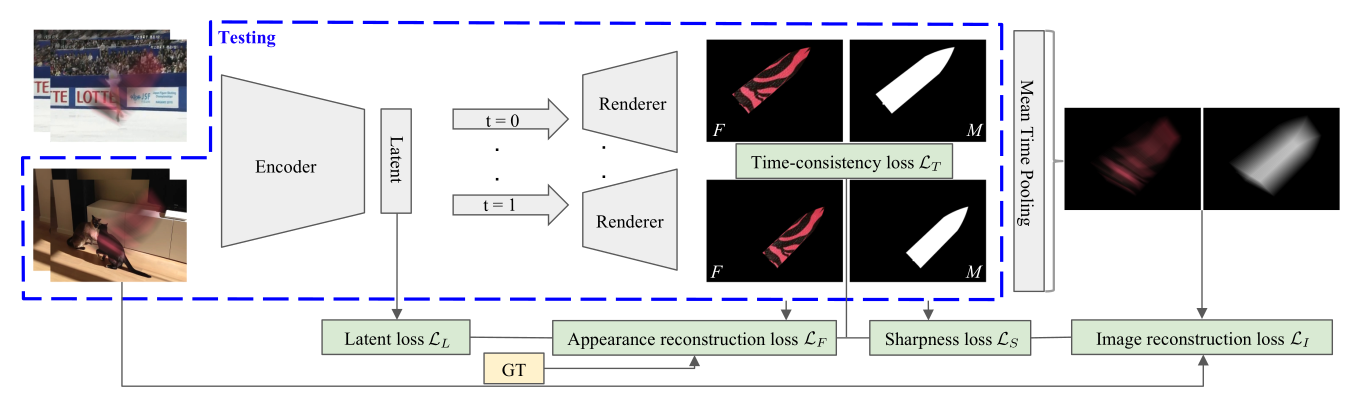
\includegraphics[width=\textwidth]{images/defmo-arch.png}
    \caption{Architecture of DeFMO.}%
    \label{fig:defmo-arch}
\end{figure}

\paragraph{Architecture}
DeFMO uses an encoder to encode $I$ and $B$ into a latent vector $X \in \mathbb{R}^K$.
The encoder is a CNN that takes both $I$ and $B$ concatenated along the channel axis.
A renderer takes $X$ and time indices $t_0, t_1, \ldots, t_{N-1}$ to output the $N$ sub-frames.
This is also a CNN that uses sub-pixel convolutions~\citep{pixelshuffle}, also known as pixel shuffles, for upsampling.
An illustration of the architecture is shown in Figure~\ref{fig:defmo-arch}.

\subsection{Training losses}
    DeFMO uses a wide variety of losses to optimize the model.
    These consist of the output reconstruction loss ($\mathcal{L}_F$), the input reconstruction loss (based on Equation~\ref{eq:defmo-blatting}) ($\mathcal{L}_I$), and losses to constraint the output to have smooth movements in time ($\mathcal{L}_T$), sharp objects ($\mathcal{L}_S$), and invariance to the background ($\mathcal{L}_L$).
    Therefore, the total loss is a weighted sum of these losses:
    % TODO: Add subscript to total loss, because this is DeFMO's total loss, not our total loss
    \begin{equation}
        \mathcal{L} = \mathcal{L}_F + \alpha_I \mathcal{L}_I + \alpha_T \mathcal{L}_T + \alpha_S \mathcal{L}_S + \alpha_L \mathcal{L}_L
    \end{equation}

    \paragraph{Appearance reconstruction loss}
    $\mathcal{L}_F$ is the supervised loss for the output sub-frames.
    However, since the model has to generate movement based on a single image as the input, the movement can be in either the same direction as the ground-truth or the opposite.
    Therefore, the supervised loss $\mathcal{L}_R$ is calculated for both directions, and $\mathcal{L}_F$ is the minimum of these:
    \begin{equation}
        \mathcal{L}_F({\{ R_t, \tilde{R}_t \}}_1^N) = \frac{1}{N} \min \left( \sum_{t=1}^N \mathcal{L}_R(R_t, \tilde{R}_t) dt, \sum_{t=1}^N \mathcal{L}_R(R_t, \tilde{R}_{1-t}) dt \right)
    \end{equation}

    $\mathcal{L}_R$ for the output rendering $R_t$ and the ground-truth $\tilde{R}_t$ at time $t$ is calculated as:
    \begin{equation}
    \begin{split}
        \mathcal{L}_R(R_t = (F_t, M_t), \tilde{R}_t = (\tilde{F}_t, \tilde{M}_t)) &= \mathcal{L}_1(M_t, \tilde{M}_t, \tilde{M}_t > 0) + \mathcal{L}_1(M_t, \tilde{M}_t, \tilde{M}_t = 0)\\
        &+ \mathcal{L}_1(F_t M_t, \tilde{F}_t \tilde{M}_t, \tilde{M}_t > 0)
    \end{split}%
    \label{eq:loss-supervised}
    \end{equation}
    where $\mathcal{L}_1(A, B, M)$ is the $\mathcal{L}_1$ loss for images $A$ and $B$ conditioned on the mask $M$:
    \begin{equation}
        \mathcal{L}_1(A, B, M) = \frac{\sum_{i, j} {|| A_{i,j} - B_{i,j} ||}_1 M_{i,j}}{\sum_{i,j} M_{i,j}}
    \end{equation}

    In Equation~\ref{eq:loss-supervised}, the first two terms are for comparing the masks $M_t$ and $\tilde{M}_t$ for the foreground and background (as given by the ground truth) separately.
    The separation is to prevent imbalance due to smaller objects in a large background.
    The third term is for the object, but evaluated only in the foreground to disentangle the mask and the object channels.

    \paragraph{Image reconstruction loss}
    $\mathcal{L}_I$ is just an application of the blatting equation in Equation~\ref{eq:defmo-blatting}.
    Thus, this loss is just the $\mathcal{L}_1$ loss between the blatted image and the input image $I$:
    % TODO: L1 loss is a norm, so don't use comma
    \begin{equation}
        \mathcal{L}_I({\{ R_t \}}_1^N, I) = {\left|\left| I, \frac{1}{N} \sum_{t=1}^N F_t M_t + \left( 1 - \frac{1}{N} \sum_{t=1}^N M_t \right) B \right|\right|}_1
    \end{equation}

    \paragraph{Time-consistency loss}
    $\mathcal{L}_T$ captures the temporal smoothness of the $N$ output sub-frames.
    Informally, we want the sub-frames for nearby $t$ to be similar to each other.
    This similarity is formalized by the maximum value of the normalized cross-correlation over all pixels.
    Thus, the loss is:
    % TODO: It's N-1, not N, because t+1 for N doesn't exist
    \begin{equation}
        \mathcal{L}_T({\{R_t\}}_1^N) = 1 - \frac{1}{N} \sum_{t=1}^N \mathrm{maxncc}(R_t, R_{t+1})
    \end{equation}

    \paragraph{Sharpness loss}
    Here, $\mathcal{L}_S$ only focuses on the sharpness of the mask, and not the object contents itself.
    The mask is expected to be binary in most of the image, except at the boundaries.
    However, we simplify this constraint to just enforcing binary values.
    This is expressed by the per-pixel binary entropy $\mathcal{H}_2$ averaged over all $H \times W$ pixels:
    \begin{equation}
        L_S({\{M_t\}}_1^N) =  \frac{1}{NHW} \sum_{t=1}^N \sum_{i=1}^H \sum_{j=1}^W \mathcal{H}_2({[M_t]}_{i,j})
    \end{equation}

    \paragraph{Latent learning loss}
    $\mathcal{L}_L$ aims to constrain the model such that blurred images of the same FMO moving along the same trajectory but in front of different backgrounds generate the output.
    This can be achieved by modelling the latent space such that these images have the same latent representation.
    Thus, DeFMO trains in pairs of such images, and computes $\mathcal{L}_L$ between their latent vectors $X_1, X_2 \in \mathbb{R}^K$as:
    \begin{equation}
        \mathcal{L}_L(X_1, X_2) = \frac{{|| X_1 - X_2 ||}_1}{K}
    \end{equation}

    Note that not all losses used here are unbiased, especially the time-consistency and sharpness losses.
    The ground-truth renderings won't necessarily be the minimum of these losses individually, since the time-consistency loss prefers static sub-frames, and the sharpness loss prefers binary masks everywhere, even on boundaries.
    This brings us to our proposed approach, where we want to overcome these limitations and get more general losses.

\section{Proposed approach}

\subsection{GANs}
    % TODO: Explain GANs independent of DeFMO
    We use GANs to replace the sharpness loss.
    In the GAN framework, there are two models, a generator and a discriminator, that compete against each other in a zero-sum game.
    The goal is to train the generator to generate data when given a dataset, in an unsupervised learning setting.
    % TODO: Why using 'ground-truth' in an unsupervised learning setup?
    The discriminator has to distinguish between the generator's outputs and the ground-truth from the dataset.
    At convergence, we expect the generator to be able to successfully fool the discriminator by learning to generate data that is indistinguishable from the dataset.

    \paragraph{Patch discriminators}
    \citet{pix2pix} extend GANs to also work in supervised learning settings, by introducing the concept of a `patch discriminator'.
    As opposed to traditional GANs, where the discriminator outputs predictions for whole images, the patch discriminator outputs predictions for each $P \times P$ patch of the input image.
    This complements the supervised learning objective to generate more realistic output images.
    As the authors point out, the supervised loss will capture the low-frequency features in the output data, while the discriminator will capture the high-frequency features.

\subsection{Sharpness loss}
    Since we already have a supervised loss for the outputs ($\mathcal{L}_F$), we use a patch discriminator for the sharpness loss.
    The main model is now viewed as a generator.
    The discriminator $D_S$ is a CNN that takes as input an RGBA image $R \in \mathbb{R}^{H \times W \times 4}$ with the same structure and representation as the outputs of the generator.
    It will output a scalar prediction for each $P \times P$ patch in the image, which are averaged to get the output for the entire image.
    The new architecture is shown in Figure~\ref{fig:gan-arch}.

    \begin{figure}
        \centering
        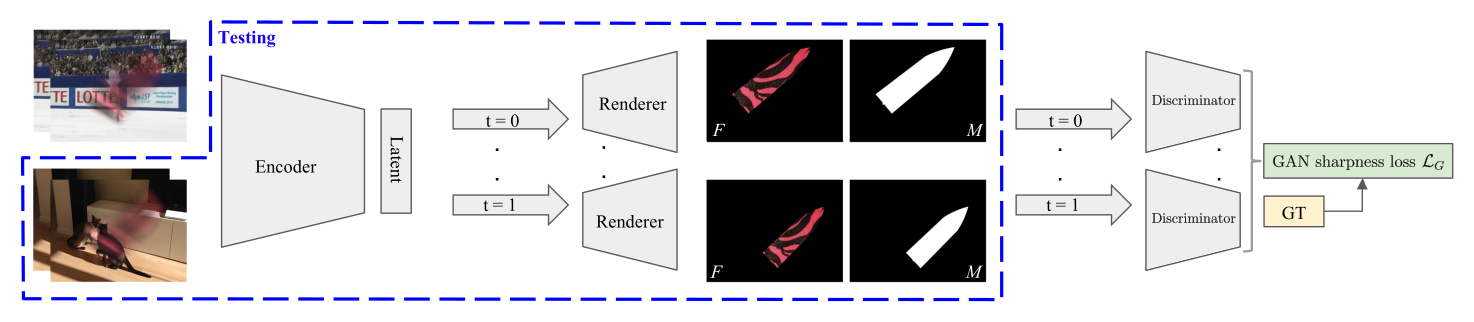
\includegraphics[width=\textwidth]{images/gan-arch.png}
        \caption{
            Architecture for the GAN-based sharpness loss.
            The discriminator takes as input one complete sub-frame and predicts whether each $P \times P$ patch is valid or not.
        }%
        \label{fig:gan-arch}
    \end{figure}

    We use the Wasserstein loss~\citep{wgan} to train the GAN.\@
    This loss requires $D_S$ to be a 1-Lipschitz function.
    We use spectral normalization~\citep{spectral-norm} over all of its weights to enforce this constraint.
    Thus, the new GAN-powered sharpness loss $\mathcal{L}_G$ is:
    \begin{equation}
        \mathcal{L}_G({\{ R_t, \tilde{R}_t \}}_1^N) = \frac{1}{N} \sum_{t=1}^N \left( \mathbb{E}_{\tilde{R}_t}[D_S(\tilde{R}_t)] - \mathbb{E}_{R_t}[D_S(R_t)] \right)
    \end{equation}

    Here, the expectation is approximated by a mean over a batch of inputs.
    The objective for $D_S$ is to maximize this loss, whereas the generator has to minimize this.

    Intuitively, $D_S$ will focus on the high-frequency features of each sub-frame $R_t$ --- both the foreground $F_t$ and the mask $M_t$.
    This means that both the texture of the foreground object and the sharpness of the boundaries must be optimal.
    Since $D_S$ can learn a highly non-linear function, $\mathcal{L}_G$ improves over $\mathcal{L}_S$ in the following ways:
    \begin{itemize}
        \item It incorporates foreground details.
        \item It can identify boundaries and thus relax the constraint of binary mask values near them.
        \item It can enforce spatial continuity of mask values --- entropy has no spatial knowledge.
        \item It is general enough to be used in other tasks involving fine-grained image details.
    \end{itemize}

\subsection{Time-consistency loss}
    Here, we modify the objective for the discriminator to distinguish between consecutive frames and random frames.
    The input to this discriminator $D_T$ is a pair of RGBA images $R_1, R_2 \in \mathbb{R}^{H \times W \times 4}$ with each RGBA image having the same structure and representation as the outputs of the generator.
    $D_T$ is a CNN that will be given all possible pairs of output sub-frames, and it has to identify if $R_2$ immediately follows $R_1$.

    Therefore, if either all sub-frames are identical or lack temporal smoothness, then the discriminator cannot distinguish them.
    The only optimum is to have proper temporal smoothness.
    Thus, this loss improves over the previous time-consistency loss since it enforces smooth movement, whereas the previous loss encourages static sub-frames.
    Further, unlike the GAN sharpness loss, this is a self-supervised setup that doesn't need any ground-truth.

    However, unlike the sharpness loss, we cannot use the GAN framework here.
    This is because we want \textbf{both} the discriminator and the generator to optimize this.
    Since the two networks need to help each other, this is not a GAN.\@
    Therefore, we simply model this loss using binary cross-entropy:
    \begin{equation}
        \mathcal{L}_N = - \frac{1}{N^2} \sum_{t=1}^N \sum_{u=1}^N \left( \mathbbm{1}[u=t+1] \log D_T(R_t, R_u) + \mathbbm{1}[u \neq t+1] \log (1 - D_T(R_t, R_u)) \right)
    \end{equation}

    % TODO: Maybe explain perceptual losses?
    This is a novel loss function that can be thought of as a neural-network-based learned loss.
    The architecture for this setup is shown in Figure~\ref{fig:temp-nn-arch}.

    \begin{figure}
        \centering
        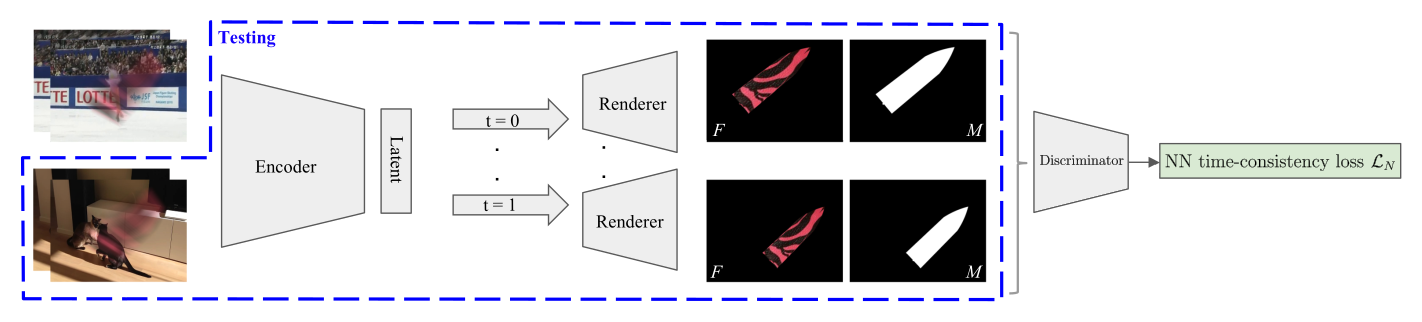
\includegraphics[width=\textwidth]{images/temp-nn-arch.png}
        \caption{
            Architecture for the NN-based time-consistency loss.
            The discriminator takes as input each possible pair of sub-frames separately and predicts whether the second one follows the first.
        }%
        \label{fig:temp-nn-arch}
    \end{figure}

% TODO: Explain how the new total loss is

\section{Experiments}

\subsection{Dataset}
    The models are trained on the synthetic dataset introduced by \citet{defmo}, due to lack of a large and diverse real-world annotated dataset with FMOs.
    Each synthetic image consists of an \textit{object}, a 6D \textit{trajectory}, and a \textit{background} frame.
    \textit{Objects} are sampled from 3D models of the 50 largest classes in the ShapeNet~\citep{shapenet} dataset.
    \textit{Trajectories} are sampled uniformly as a combination of 3D linear translations and 3D rotations.
    \textit{Backgrounds} are sampled from the VOT~\citep{vot} sequences for training, and from Sports-1M~\citep{sports-1m} for validation.

    For evaluation, the models are evaluated on several datasets using the open source FMO deblurring benchmark introduced by \citet{defmo} using ideas taken from \citet{fmo}.
    It includes the Falling Objects~\citep{falling-objs}, TbD-3D~\citep{tbd-3d}, and TbD~\citep{tbd} datasets.

\subsection{Architecture}
    The encoder and both discriminators have the ResNet-18~\citep{resnet} architecture (up to and excluding the global average pooling layer), and their weights are initialized with a model pre-trained on ImageNet~\citep{imagenet}.
    Thus, the latent space is of 512 dimensions (due to ResNet-18).
    The parameters of the first layer are adapted to the no.\ of channels in the inputs by duplicating the pre-trained weights.

    The discriminators use spectral normalization~\citep{spectral-norm} to stabilize training, and to enforce the 1-Lipschitz constraint for the Wasserstein loss~\citep{wgan} in the GAN sharpness loss.
    $D_S$ has a convolution layer without any non-linearity after the ResNet-18 backbone, after which global average pooling combines the patch predictions into a single scalar.
    Here, since ResNet-18 downsamples the input images by 32, therefore the patch size will be $(\lceil H/32 \rceil, \lceil W/32 \rceil)$.
    $D_T$ keeps the global average pooling layer after the ResNet-18 backbone, and adds a fully-connected layer with sigmoid activation on top of the pooling layer with a scalar output.

    The renderer is a standard CNN with batch normalization~\citep{batch-norm} and ReLU~\citep{relu}.
    Additionally, it uses the ResNet bottleneck along with pixel shuffling~\citep{pixelshuffle} for upsampling.
    The exact architecture is shown in Table~\ref{tab:renderer-arch}.

    \begin{table}
        \caption{
            Architecture of the renderer.
            Parameter values correspond to those used in PyTorch v1.8 for the corresponding layers.
        }%
        \label{tab:renderer-arch}
        \centering
        \begin{tabular}{llll}
            \toprule
            Layer & Channels & Kernel size & Stride\\
            \midrule
            Conv2d & 1024 & 3 & 1\\
            BatchNorm2d & 1024\\
            ReLU\\
            ResNet bottleneck & 256\\
            PixelShuffle &&& 2\\
            ResNet bottleneck & 64\\
            PixelShuffle &&& 2\\
            ResNet bottleneck & 16\\
            PixelShuffle &&& 2\\
            Conv2d & 16 & 3 & 1\\
            PixelShuffle &&& 2\\
            Conv2d & 4 & 3 & 1\\
            ReLU\\
            Conv2d & 4 & 3 & 1\\
            \bottomrule
        \end{tabular}
    \end{table}

    We compare our proposed approach to our re-implementation of DeFMO.\@
    Here, we reduce the number of parameters in DeFMO by swapping ResNet-50 for ResNet-18 in the encoder and by appropriately reducing the number of neurons in the first layer of the decoder.
    Then, we re-train the model with a different set of hyper-parameters.

\subsection{Setup}
    The models are trained using the Adam~\citep{adam} optimizer.
    There is one optimizer for the main model (encoder and renderer), one for $D_S$ and one for $D_T$.
    Optimization steps for $D_S$, $D_T$, and the main model are taken alternately.
    Step-wise learning rate decay is applied for all optimizers.

    The code was written in Python using the PyTorch~\citep{pytorch} library.
    It was run on a cluster that uses CUDA~\citep{cuda} on three NVIDIA GeForce\textsuperscript{\textregistered} GPUs with 11 GiB memory for accelerating PyTorch.

    Hyper-parameters were manually chosen --- no hyper-parameter search procedure was used.
    Their values are shown in Table~\ref{tab:hyper-params}.

    \begin{table}
        \caption{
            Hyper-parameter values used for our re-implementation of DeFMO and our proposed approach.
            Any missing values are assumed to have the defaults as in PyTorch v1.8.
            Hyphen denote that values aren't applicable.
        }%
        \label{tab:hyper-params}
        \centering
        \begin{tabular}{lrr}
            \toprule
            \multirow{2}[2]{*}{Name} & \multicolumn{2}{c}{Approach}\\
            \cmidrule(lr){2-3}
            & DeFMO (ours) & Proposed\\
            \midrule
            Epochs & \defmoepochs{} & \oursepochs\\
            Batch size & \defmobatchsize{} & \oursbatchsize\\
            Input resolution & 128$\times$128 & 128$\times$128\\
            Number of sub-frames ($N$) & 24 & 24\\
            Learning rate (main model) & 0.001 & 0.001\\
            Learning rate ($D_S$) & - & 0.00001\\%chktex 8
            Learning rate ($D_T$) & - & 0.00005\\%chktex 8
            Learning rate decay rate (all schedulers) & 0.5 & 0.5\\
            Learning rate decay step size (all schedulers) & 10 & 10\\
            $D_S$ steps per main model step & - & 1\\%chktex 8
            $D_T$ steps per main model step & - & 2\\%chktex 8
            Image reconstruction loss weight ($\alpha_I$) & 1.0 & 1.0\\
            Time-consistency loss weight ($\alpha_T$) & 1.0 & -\\
            Sharpness loss weight ($\alpha_S$) & 1.0 & -\\
            Latent learning loss weight ($\alpha_L$) & 1.0 & 1.0\\
            GAN sharpness loss weight ($\alpha_G$) & - & 1.0\\%chktex 8
            NN-based time-consistency loss weight ($\alpha_N$) & - & 0.05\\%chktex 8
            \bottomrule
        \end{tabular}
    \end{table}

\subsection{Memory optimizations}\label{sec:mem-opt}
    A disadvantage of our approach is that the addition of discriminators increases compute and memory usage significantly.
    Therefore, we adopt a few techniques to reduce the GPU memory impact.

    \paragraph{Gradient checkpointing}
    This technique trades computation for lower memory usage.
    \citet{grad-ckpt} introduce gradient checkpointing, an algorithm that can train an $n$ layer network with $\mathcal{O}(\sqrt(n))$ memory cost.
    Simply put, it replaces intermediate activations by `checkpoints'.
    When a checkpoint is later needed during back-propagation, the activations are recomputed.
    Thus, the memory savings come at the cost of extra forward passes per mini-batch.

    \paragraph{Mixed precision training}
    This technique trades accuracy for faster computation and lower memory usage.
    Training networks using 32-bit single-precision floating points is typically more compute- and memory-intensive than 16-bit half-precision floats.
    However, using half-precision may lead to training instability due to underflow in gradients.
    \citet{amp} introduce mixed-precision training, a technique that uses half-precision for all computations that aren't sensitive to precision, and single-precision otherwise.
    To avoid underflow in gradients, it also scales losses before calculating gradients, and unscales the gradients when applying them.

\newcommand{\samples}[2]{%
    \begin{figure}
        \centering

        \begin{subfigure}{0.19\textwidth}
            \includegraphics[height=\textwidth,width=\textwidth]{images/results/#1.jpg}
            \caption*{Input}
        \end{subfigure}
        \hfill
        \begin{subfigure}{0.79\textwidth}
            \setlength{\abovecaptionskip}{1mm}
            \foreach [count=\i from 1] \method/\name in {GT/gt,DeFMO/old,Ours/new}{%chktex 1
                \begin{subfigure}{\textwidth}
                    \rotatebox{90}{\method}
                    \foreach \j in {0,...,7}{%chktex 1,chktex 11
                        \includegraphics[height=0.11\textwidth,width=0.11\textwidth]{images/results/\name/#1-\j.jpg}%
                        \ifthenelse{\equal{\j}{7}}{}{\hfill}%
                    }
                \end{subfigure}%
                \ifthenelse{\equal{\i}{3}}{}{\vspace{1mm}}
            }
            \caption*{Output}
        \end{subfigure}

        \caption{Sample outputs on the #2 dataset.}%
        \label{fig:#1-samples}
    \end{figure}
}

\section{Results}

\subsection{Benchmark results}
    The FMO deblurring benchmark evaluates the models using peak signal-to-noise ratio (PSNR), structural similarity index measure~\citep{ssim} (SSIM), and intersection over union averaged over the trajectory~\citep{tiou} (TIoU).
    Here, both methods use a median of the previous five frames as the background.
    The results for this benchmark are shown in Table~\ref{tab:benchmark}.
    Image samples on the Falling Objects, TbD-3D and TbD datasets are shown in figures \ref{fig:falling-objs-samples}, \ref{fig:tbd-3d-samples} and \ref{fig:tbd-samples} respectively.%chktex 2

    % TODO:
    % * Specify that this is the re-implemented DeFMO
    % * Specify metrics for original DeFMO
    % * Do ablation study
    \begin{table}
        \caption{
            Evaluation on the FMO deblurring benchmark.
            The datasets are sorted top-to-bottom by decreasing difficulty: arbitrary shaped and textured~\citep{falling-objs}, mostly spherical but textured~\citep{tbd-3d}, and mostly spherical and uniformly coloured objects~\citep{tbd}.
        }%
        \label{tab:benchmark}
        \centering
        \begin{tabular}{llrr}
            \toprule
            \multirow{2}[2]{*}{Dataset} & \multirow{2}[2]{*}{Metric} & \multicolumn{2}{c}{Approach}\\
            \cmidrule(lr){3-4}
            && DeFMO & Ours\\
            \midrule
            \multirow{3}{*}{Falling Objects} & TIoU $\uparrow$ & 0.000 & 0.000\\
            & PSNR $\uparrow$ & \textbf{22.794} & 22.064\\
            & SSIM $\uparrow$ & \textbf{0.608} & 0.604\\
            \midrule
            \multirow{3}{*}{TbD-3D} & TIoU $\uparrow$ & 0.000 & 0.000\\
            & PSNR $\uparrow$ & 20.156 & \textbf{21.256}\\
            & SSIM $\uparrow$ & 0.533 & 0.533\\
            \midrule
            \multirow{3}{*}{TbD} & TIoU $\uparrow$ & 0.000 & 0.000 \\
            & PSNR $\uparrow$ & 20.262 & \textbf{20.947} \\
            & SSIM $\uparrow$ & 0.471 & \textbf{0.511}\\
            \bottomrule
        \end{tabular}
    \end{table}

    \samples{falling-objs}{Falling Objects}
    \samples{tbd-3d}{TbD-3D}
    \samples{tbd}{TbD}

    % TODO: Specify that this is re-implemented DeFMO
    As we can see, our approach performs better than DeFMO in the TbD-3D and TbD datasets.
    In the Falling Objects dataset, it falls short of DeFMO.\@
    This is presumably because of insufficient training for our model (\oursepochs{} epochs for ours vs \defmoepochs{} epochs for DeFMO, as shown in Table~\ref{tab:hyper-params}), although neither model is trained till convergence (due to lack of time).
    Both models get 0.000 TIoU, further reinforcing the previous remark.

    Further, due to memory limitations, the maximum batch size achievable for our approach was \oursbatchsize, lower than that for DeFMO (which is \defmobatchsize).
    Since we build upon ResNet-18, which uses batch normalization, lower batch sizes impact accuracy.
    Hence, with more time and more GPU memory, our approach should outperform DeFMO.\@

\subsection{Memory optimizations}
    The memory savings due to techniques in Section~\ref{sec:mem-opt} are shown in Table~\ref{tab:mem-opt}.
    Memory usage is calculated using a custom wrapper around the NVIDIA System Management Interface~\citep{nvidia-smi} (\texttt{nvidia-smi}) tool, which is included with NVIDIA's GPU drivers.
    Here, the training is stopped after two gradient steps.
    Also, all hyper-parameters are the same as in Table~\ref{tab:hyper-params}, except for batch size, which is 5.

    \begin{table}
        \caption{
            Ablation study for memory usage (in MiB) across both approaches during training on a single GPU.\@
            We use gradient checkpointing with 2 segments over the encoder and renderer separately.
        }%
        \label{tab:mem-opt}
        \begin{tabular}{lrrrr}
            \toprule
            \multirow{2}[2]{*}{Technique} & \multicolumn{4}{c}{Approach}\\
            \cmidrule(lr){2-5}
            & DeFMO & $+ D_S$ & $+ D_T$ & $+ D_S, D_T$\\
            \midrule
            None & 2413 & 6351 & 6211 & 10023\\
            Gradient checkpointing (GC) & 2121 & 5933 & 5965 & 9803\\
            Mixed precision (MP) & 1807 & 4003 & 3997 & 6073\\
            GC + MP & \textbf{1667} & \textbf{3909} & \textbf{3835} & \textbf{5991}\\
            \bottomrule
        \end{tabular}
        \centering
    \end{table}

    Evidently, our model consumes much more memory than DeFMO.\@
    However, the gap can be reduced considerably by both gradient checkpointing and mixed precision.
    While both significantly reduce memory usage, mixed precision gives a larger improvement.

\subsection{Code quality}
    Code quality is assessed using Cyclomatic Complexity~\citep{mccabe} (CC), Halstead~\citep{halstead} difficulty and delivered bugs, and the Maintainability Index~\citep{mi-original,mi-revision} (MI).
    These were calculated using the open source tool Radon~\citep{radon} on the current source code (as of commit \texttt{cc4a28106ca0332e8cbca17504ff6691288578a7}) and the original DeFMO repository (at the commit it was forked: \texttt{30c5af80e49c96d39090c4b51541cd6801d2934a}), excluding the code for rendering the synthetic dataset.
    The extrema and average values of these metrics are presented in Table~\ref{tab:radon}.

    \begin{table}
        \caption{Code quality comparison between original DeFMO and this project.}%
        \label{tab:radon}
        \centering
        \begin{tabular}{lrrrrrrrr}
            \toprule
            \multirow{2}[2]{*}{Approach} & \multicolumn{2}{c}{CC $\downarrow$} & \multicolumn{2}{c}{Difficulty $\downarrow$} & \multicolumn{2}{c}{Bugs $\downarrow$} & \multicolumn{2}{c}{MI $\uparrow$}\\
            \cmidrule(lr){2-3} \cmidrule(lr){4-5} \cmidrule(lr){6-7} \cmidrule(lr){8-9}
            & Avg & Max & Avg & Max & Avg & Max & Avg & Min\\
            \midrule
            DeFMO & 4.647 & 78 & 7.030 & 13.852 & 0.480 & 2.228 & 44.89 & 8.19\\
            Ours & \textbf{3.349} & \textbf{15} & \textbf{5.149} & \textbf{9.960} & \textbf{0.209} & \textbf{0.589} & \textbf{48.86} & \textbf{23.24}\\
            \bottomrule
        \end{tabular}
    \end{table}

    As we can see, the refactoring done on the code base has significant improvement over the previous state, especially when considering the extrema of these metrics.

\section{Conclusion}

We proposed an improved version of DeFMO that uses GANs to overcome its problems with biased losses.
We also proposed a novel loss function to capture smooth movement across sub-frames.
This method can also generalize better to other related applications, like temporal super-resolution, due to more general loss functions.
% TODO: Explain that this is referring to the re-implementation of DeFMO
Experimental results show that the proposed model performs better than DeFMO on their benchmark, but at the cost of higher memory usage during training.
We also implement popular memory optimization techniques and refactor the codebase to make is easier to use, maintain, and extend the approach.
% TODO: Explain that achieving SoTA is due to beating original DeFMO, not re-implemented DeFMO
For future work, one can train the model on full resolution images with sufficient compute to possibly achieve state-of-the-art results.


\small
\bibliography{references}

\end{document}
